\chapter{Design}\label{chap:Design}\todo{i wonder whether design + architecture section should be merged. the thing is that design is more about concrete design decisions (which are more related to implementation) whereas architecture is abstract and conceptual.}

This section goes over the initial design for the solution we present. Any major deviations from this design are noted in Chapter~\ref{chap:Implementation}. To make design decisions, we re-evaluate the functional requirements taking into account the techniques gleaned and the lessons learnt from Background and Related Work

\section{Static vs Dynamic}

The first and largest choice faced is whether to use dynamic or static detouring for our library. After deciding this, we can evaluate the available implementation options.

Even though implementing detouring at runtime offers advantages such as flexibility and ease of development, it was ruled out as an option because we did not find a dynamic method which does not compromise \emph{(F6)}. That is, all the runtime methods we have looked at require some form of environment, whether this is through the distribution of a shared library, process-level virtual machine or otherwise. Since a dynamic solution is infeasible, we can narrow the scope of the solution to the various static binary rewriting approaches.

\section{Proposed Workflow}

In order to make further design decisions, we take a top-down design approach. We first define the expected workflow with a tool created with our library. After this is decided, we can fledge out the design details for the implementation of each stage of this workflow. Figure~\ref{fig:Workflow} illustrates the proposed workflow of our library according to the exemplary model described in Chapter~\ref{chap:Introduction}.

The approach results in a workflow that is in part similar to that of EEL. The similarity lies in the fact that we also inject an object file. However, because we are only targeting x86-32 and x86-64, we can make improvements in the following areas:

\begin{description}
\item[Expressibility] EEL caters for many architectures and for this reason, requires users to directly write small chunks of assembly which will be patched into the executable. While it is useful to expose such functionality, it would be convenient to abstract away entirely from assembly language. Since we are only targeting two architectures, there is no need to expose such general functionality. Even if we do choose to expose it, we can do better by providing a rich API for detouring and trampolining specifically since this is the main focus. It is important to note that the main focus of the library is detouring, so having a more specific API which is less cumbersome but narrower may well be preferable to having a very general one that allows everything to be done.
\item[Overhead] We can try to address the problem of overhead in object insertion. To recap, the reason for the overhead is that when an object is inserted, all its dependencies are also recursively inserted, which are required to be statically linked. The problem with this is that if the object file is linked against libc, then a copy of the entire libc library will be bundled into the binary upon injection. Theoretically, this should not be necessary if the target is already linked against libc (whether dynamically or statically). If this is the case, it would be redundant to pull in an extra copy of the library. We should not be limited by the fact that EEL decided to take this route and instead we should investigate alternatives that allow object injection that does not duplicate dependencies.
\end{description}

\begin{figure}[H]
 \centering
 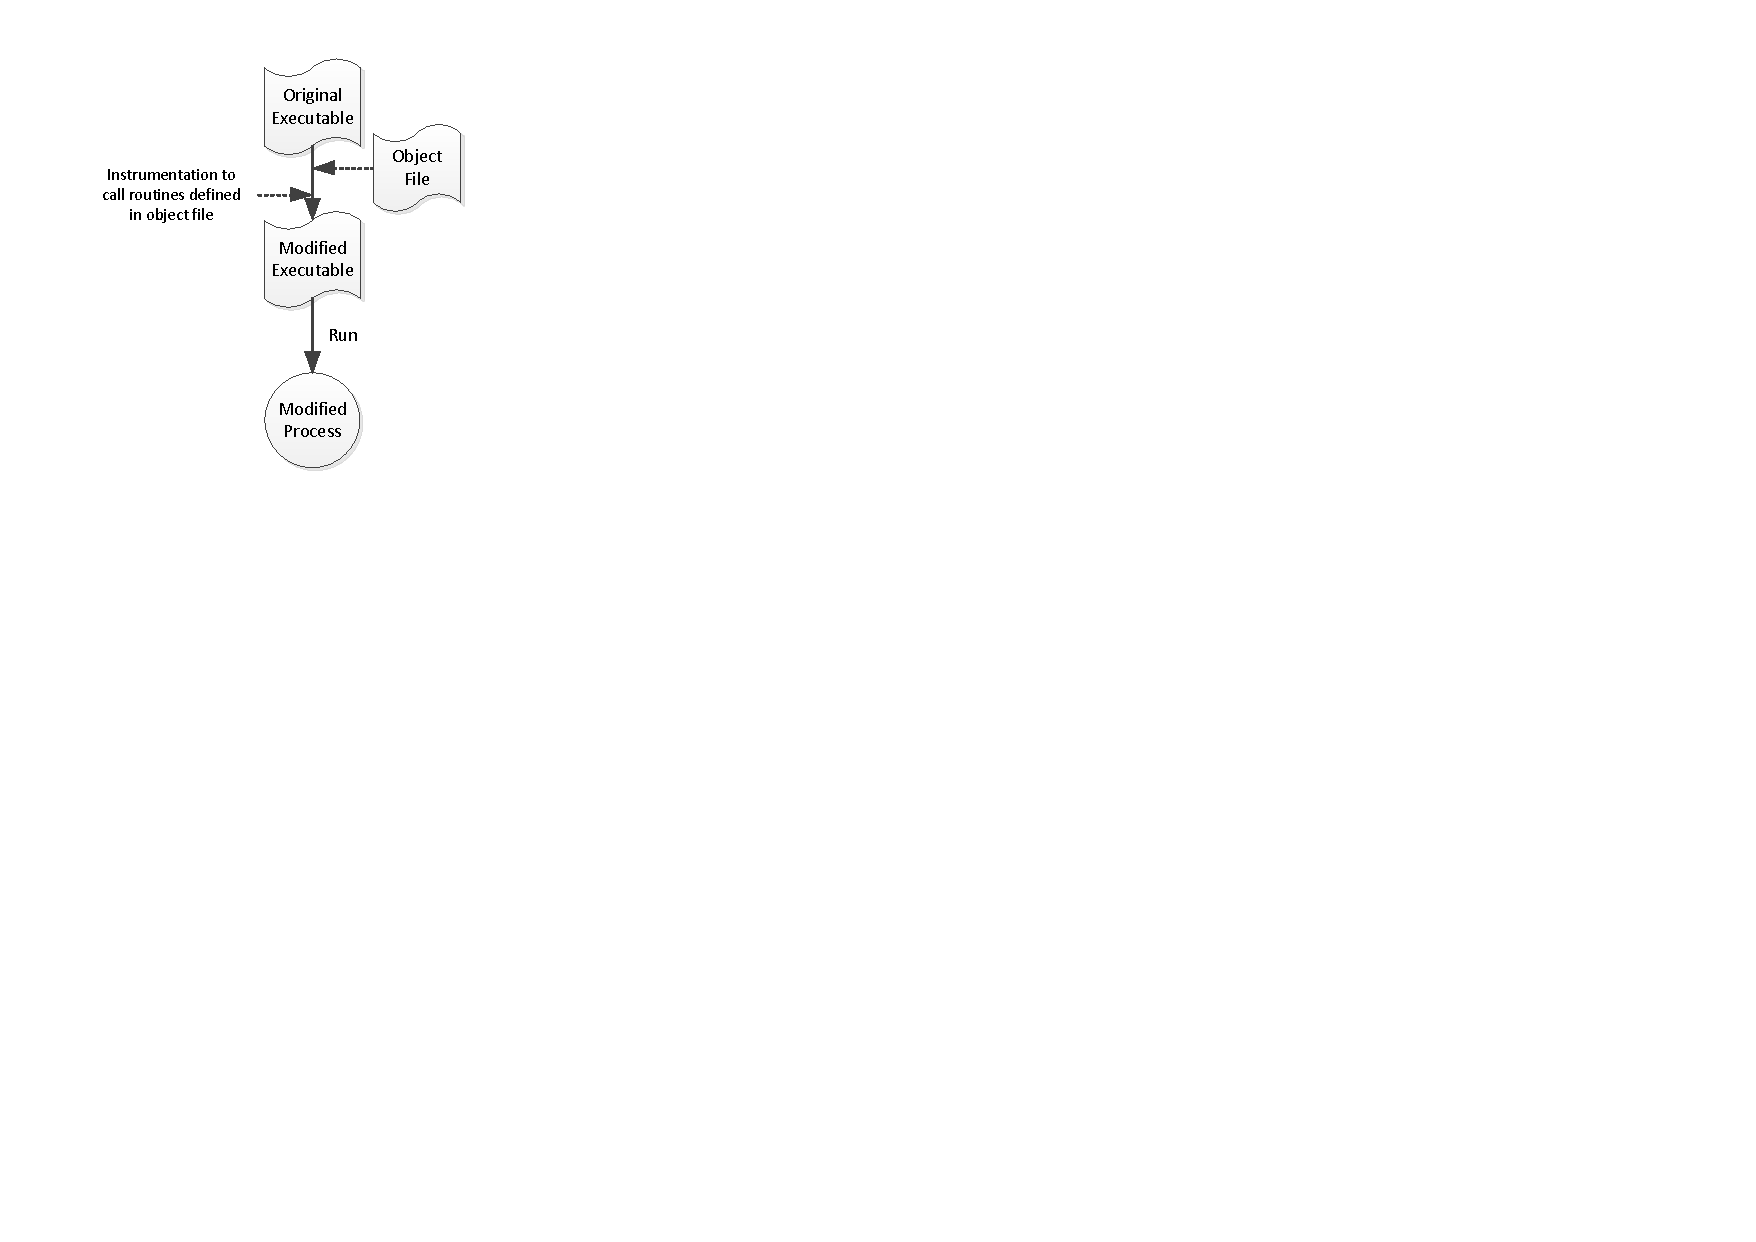
\includegraphics{Workflow.pdf}
 \caption[Hierarchy]{The proposed method for instrumentation. An object file containing user defined routines is optionally injected into the target binary. Using binary rewriting, the original code is then connected to the injected code.}
\label{fig:Workflow}
\end{figure}

From the proposed workflow, it can be seen that there are two distinct phases:

\begin{description}
\item [Object injection] This phase will take as input the original binary and an object file and output a new binary which is the result of a merge of the two inputs. This satisfies \emph{(F6)}.
\item [Binary rewriting] This will be used to statically patch detours and trampolines into the binary. This satisfies \emph{(F1)}, \emph{(F2)} and \emph{(F6)}.
\end{description}

On top of this, we add one more phase:

\begin{description}
\item [Binary analysis] We borrow the concept from Etch of having a code discovery stage. This will allow users to select what function or basic block they are going to detour/trampoline. This binary analysis should also produce the CFG that is required by \emph{(F4)} and \emph{(F5)}.
\end{description}

\emph{(F7)} is an implementation detail, which will be discussed in Implementation (Chapter~\ref{chap:Implementation}).

\section{Static Analysis Engine}

The static analysis engine corresponds to the binary analysis stage mentioned above. To re-iterate, the aim of the static analysis engine is to generate a CFG from a binary and expose an interface to it. The user will iterate the discovered basic blocks and functions, choosing one to instrument. Providing such functionality will require a disassembler engine.

\subsection{Disassembler Engine}

Creating our own disassembler engine is an option, but that is unnecessary given the number of implementations already existing. It would be convenient to use a disassembler that can disassemble both x86-32 and x86-64 as opposed to building on top of two separate disassemblers. \emph{libopcodes} provides functionality to disassemble executable binaries into human readable formats. Many of the GNU binutils programs use the opcodes library to assemble and disassemble machine instructions. This makes it a natural choice because it is guaranteed to be heavily ported and readily available. Although portability is not a key concern, there is no reason to block that option in case the library is ported in the future. It can be considered a bonus that if we decided to port our library to another architecture, it is likely the disassembler engine could be reused. Another slightly related advantage is that libopcodes takes as input a BFD object (as opposed to a native ELF file). This means we can abstract from libelf, which we want to avoid if possible because of \emph{(F7)}. Unfortunately, libopcodes has several shortcomings:

\begin{description}
\item [Limited disassembly scope] Disassembly with the library is limited to a single address at a time (as opposed to be able to disassemble a function or basic block in a batch operation). Furthermore, some disassemblers actually provide CFG generation out of the box which means if we take this option, we will have to reproduce a CFG generator.
\item [Designed for streams] The library is designed to print to a stream. This does not make it the output amenable for storage or analysing.
\end{description}

On the other hand, libopcodes is likely to continue to be supported for the foreseeable future given that widely used binutils tools build on top of it. The most notable of these is objdump. Unfortunately, we are unable to make use of objdump because it does not support control-flow disassembly. In summary, there are several implications when considering libopcodes which we should expect to have to deal with:

\begin{description}
\item [CFG Generation] In order to generate a CFG, we need to write our own code that builds one from single instructions.
\item [Output redirection] We need to override the behaviour where libopcodes outputs to a stream. Outputting to a file and reading back from it is an unacceptable solution because of the overhead.
\end{description}

\emph{libopdis} is an existing library which wraps libopcodes to achieve exactly these core functionalities. However, we want a lightweight library so it is not optimal to build on top of libopdis. Even worse than this is the fact that libopcodes (like many disassemblers) only offers instruction information in terms of strings. In fact, even libopcodes returns strings when disassembling. This makes sense since it is designed to work with streams. String operations are inefficient and inconvenient for users so we should aim to find a solution to this problem. This means that libopdis is really only a thin wrapper around libopcodes so its functionality should not be hard to reproduce.

\section{Object File Injection}

Object file injection is possible in EEL which builds on top of BFD only, so it is reasonable to expect that the BFD library provides functionality which allows this. If this proves to be infeasible during implementation, we will need to investigate other approaches.

\section{Static Patcher}

It is convenient that we have decided to use libbfd for the static analysis engine because it is also possible to write files through libbfd. Several well known binutils tools do exactly this (for example, ld and objcopy).

\section{Summary of Design}

We propose an implementation of executable editing which works on top of the BFD library. This makes adaquate use of existing functionality as required by \emph{(F7)}. BFD will work in conjunction with the libopcodes library to produce the control flow graph as required by \emph{(F4)} and \emph{(F5)}. To inject user-defined routines, we can take a similar approach to EEL and allow the user to specify an object file to be merged with the target binary. The next step would then be to find some mechanism by which procedural-level detouring can be achieved \emph{(F1)}, again through BFD. This is the first point at which we are modifying the target's code in any way. The technique used will have to be modified slightly to accommodate for the trampolining as required by \emph{(F2)}. Since the user defined functions are compiled separately to the target, they do not know what address to call for the trampoline so this is something we will have to deal with.